\documentclass{beamer}
\usetheme{Copenhagen}

\usepackage{caption}
\usepackage{amsmath}
\title{A generalized SIR and an approach to network}
\subtitle{Efforts of a newbie}
\date{Simone Amadio}

\begin{document}
	\begin{frame}
		\titlepage
	\end{frame}



	\begin{frame}
	\title{Chapter 1: Preliminaries and model}
	\subtitle{}
	\date{}
	\titlepage
	\end{frame}


	\begin{frame}
		\frametitle{An informal definition of network}
		As long as we are concerned, a network is a set of agents in which the behaviour (transition rates/probabilities) of a single individual is affected by the state of some other agents, called neighbours.
		
		It can easily be represented by an adjacency matrix $A_{ij}$ and a set of rates. 
		
		Here the topology of the networks is fixed (no scale-free networks).
	\end{frame}



	\begin{frame}
		
		\frametitle{The model}
		
		\textbf{Generalised SIR}: Unified approach for disease and rumor spreading.Here we will only look at contact processes.\footnote{\textit{Ferraz De Arruda,Rodrigues,Cozzo,Moreno and Rodriguez}, Unifying Markov Chain Approach for Disease and Rumour Spreading in Complex Networks}
		
		\begin{figure}
			\centering
			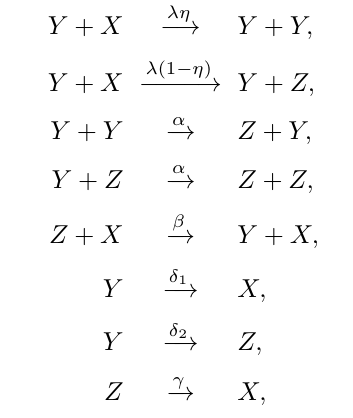
\includegraphics[width=0.4\linewidth]{transitions}
			\label{fig:transitions}
		\end{figure}
		
		
	\end{frame}

	\begin{frame}
	\frametitle{Problems of a DTMC approach}
	
	\begin{itemize}
		\item Synchronous networks
		\item Finalization $\rightarrow$ node ordering as agent/node "speed".  
	\end{itemize}

	We prevent these factors by using a CTMC approach. All the above parameters are now rates, except from $\eta$.

	\end{frame}

\begin{frame}
\title{Chapter 2: CTMC network and node-based method}
\subtitle{}
\date{}
\titlepage
\end{frame}

	\begin{frame}
\frametitle{Simulation approaches}

How to update the system? Variation of Gillespie Algorithm:

\begin{itemize}
	\item Rule-based model: total rate of a transition is match(Pattern,Graph)*single\_rate. Avoided: searching for multiple occurrences of multiple patterns in a graph can be expensive.
	\item Node-based method\footnote{\textit{St-Onge,Young,Dube'}, Efficient Sampling of spreading processes on complex networks using a composition and rejection algorithm}: the update starts from a node sampled with probability proportional to its total rate. 
\end{itemize}
\end{frame}


	\begin{frame}
	\frametitle{Node-based method with rejection sampling}
	The article analyzes the SIS model and define:
	
		\begin{itemize}
			\item $\omega_i$= total rate of interaction of node i
			\item $W=\sum_{i=1}^N \omega_i$
		\end{itemize}
	\vspace{5 pt}
	$\omega_i$ in a network depends on state of node i, rates of transitions and from $k_{i,s}$=number of neighbours of i in state s.
	
	i.e. for node(i) in state Z in our model we have $\omega_i= \gamma+k_{i,X}*\beta$ 			
	\end{frame}
	
	
	\begin{frame}
	\frametitle{Node-based method, part 2}
	 Rejection sampling is used: at every iteration the starting node j is sampled uniformly between the neighboours of i and accepted iff $rand<\omega_j/W$. Otherwise, a new node is sampled until acceptance.
	
	Let $spont_j$ be the rate of spontaneous transition of node j, let i be the accepted node, the iteration will be a spontaneous process with probability ($spont_i/\omega_i$). 
	
	Otherwise an interaction is performed, contacting a neighbour of i with uniform probability.
	\end{frame}
 	
		
	\begin{frame}
	\title{Chapter 3: Generalization and improvements}
	\subtitle{}
	\date{}
	\titlepage
	\end{frame}


\begin{frame}
	\frametitle{only Y contagion, uniform neighbour distribution}
	
	 $\lambda=\eta=1$, all the other rates are 0, so only contact from a Y nodes should be permitted.
	
	\vspace{5 pt}
	 
	 Actually the uniform neighbour sampling allows a node in state Y to contact a neighbour!=X independently of the rates, so that Y+Y$\rightarrow$ Z+Y is allowed $\forall$ rate. Z instead has no possible transition.
	
	Using $$E[N_x(it+1)]=\frac{N_x(it)}{N-1} (N_x(it)-1)+\frac{N-1-N_x(it)}{N-1} N_x(it)$$
	
	we get $$N_x(it)=N_x(0)*(1-\frac{1}{N-1})^{it}$$	
	
	The recursion for $N_y$ is more complicated and has been solved numerically.

\end{frame}

	\begin{frame}
	\frametitle{only Y contagion, uniform neighbour distribution 2}
		\begin{figure}
			\centering
			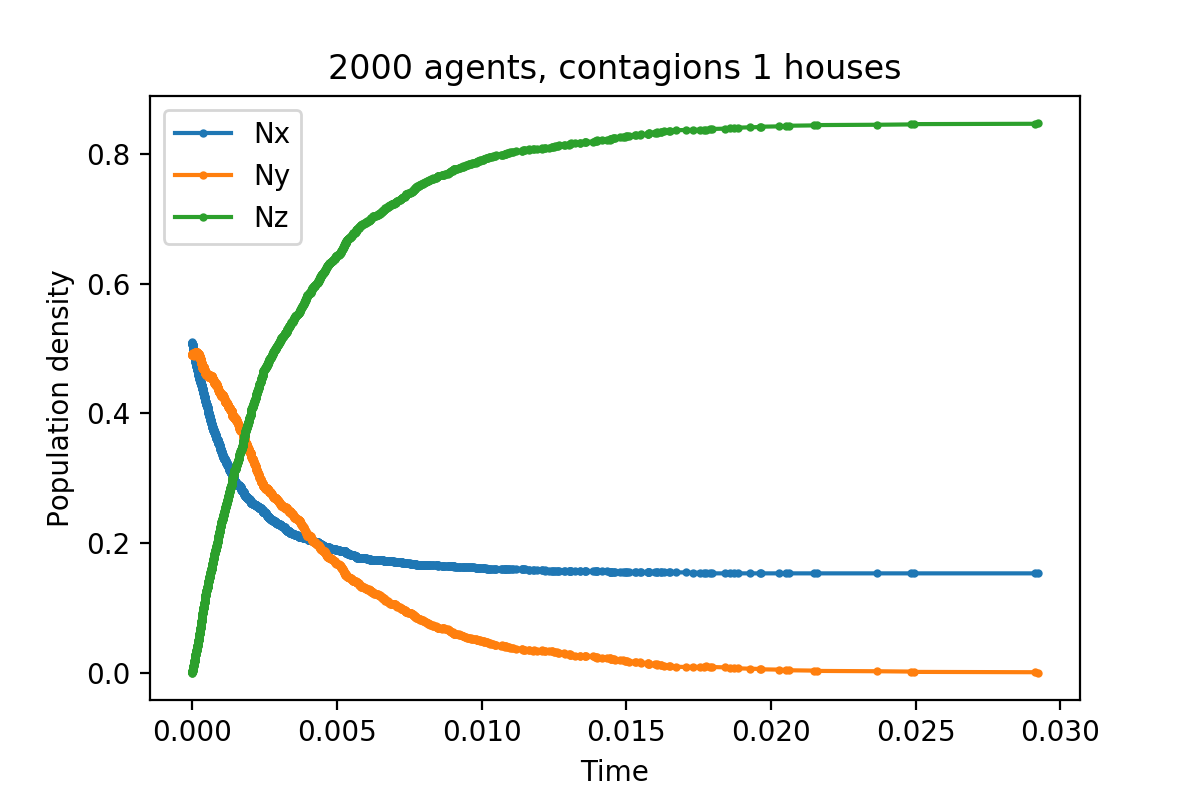
\includegraphics[width=0.5\linewidth]{only_Y_contagion_2000_complete_graph_uniform_neighbour}
			\caption*{}
			\label{fig:onlyycontagion2000completegraphuniformneighbour}
		\end{figure}
	
	Using equations from previous slides and confronting with simulated data, the relative error is $< 0.05\%$
	
	\vspace{10 pt}
	\end{frame}



	\begin{frame}
	\frametitle{Attempted improvements to node-based method}

	\begin{itemize}
		\item Generalization for multiple non spontaneous transitions.
		\item Avoid rejection sampling and directly select node using probabilities ($\omega_i/W$).
		\item Select neighbours according to rates of interaction: this also prevent the problem of independence by rate encountered in the previous slide.
	\end{itemize}
	\vspace{5 pt}
	
	\end{frame}


	
	
\end{document}